\section{Replacing \code{foreach} loops with \code{for} loops}

In Java, the \code{for} statement\footnote{\url{https://docs.oracle.com/javase/specs/jls/se8/html/jls-14.html#jls-14.14}}
has two forms: the basic one and the enhanced one. Since the meaning of the enhanced \code{for} statement is given by
translation into a basic \code{for} statement\footnote{\url{https://docs.oracle.com/javase/specs/jls/se8/html/jls-14.html#jls-14.14.2}},
the enhanced form is merely syntactic sugar for the basic one.

This pass first collects all the enhanced \code{for} statements in the method body which contain at least one recursive
call in pre-order fashion by using a visitor processing children nodes before the current node. Then it replaces these
statements by their equivalent basic \code{for} statements. This conversion is necessary because control flow needs to
be explicit for later stages in the refactoring process. The \textit{Condition} and \textit{Update} part of a \code{for}
statement in particular need to be explicit because they get executed after returning from a recursive call in the body
of the \code{for} statement.

There are two cases for this conversion: the first when the type of \textit{Expression} is a subtype of
\texttt{Iterable} (exemplified in \labelindexref{Figure}{img:foreach-to-iterator-for-before} and
\labelindexref{Figure}{img:foreach-to-iterator-for-after}) and the second when \textit{Expression} has an array type
\texttt{T[]} (exemplified in \labelindexref{Figure}{img:foreach-to-indexed-for-before} and
\labelindexref{Figure}{img:foreach-to-indexed-for-after}), where \textit{Expression} is the value over which the
enhanced \code{for} statement iterates.

\fig[height=0.5in]{src/img/foreach-to-iterator-for-before.png}{img:foreach-to-iterator-for-before}{\code{Foreach} loop to iterator \code{for} loop conversion (before)}
\fig[height=0.625in]{src/img/foreach-to-iterator-for-after.png}{img:foreach-to-iterator-for-after}{\code{Foreach} loop to iterator \code{for} loop conversion (after)}
%\fig[width=.3\textwidth]{src/img/foreach-to-indexed-for-before.png}{img:foreach-to-indexed-for-before}{\code{Foreach} loop to indexed \code{for} loop conversion (before)}
%\fig[width=.4\textwidth]{src/img/foreach-to-indexed-for-after.png}{img:foreach-to-indexed-for-after}{\code{Foreach} loop to indexed \code{for} loop conversion (before)}
\begin{figure}[htb]
    \centering
    \begin{minipage}[b]{0.45\textwidth}
        \centering
        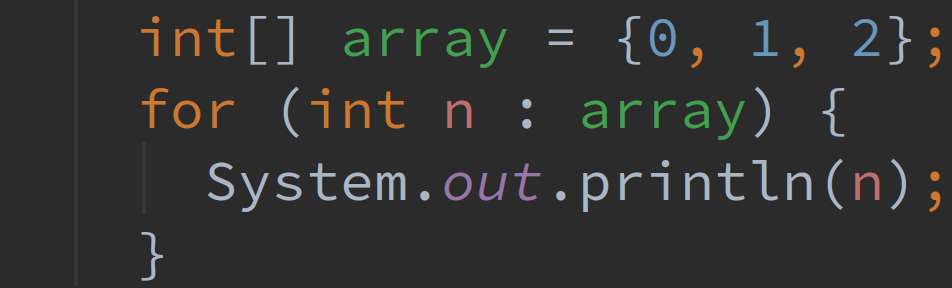
\includegraphics[height=0.5in]{src/img/foreach-to-indexed-for-before.png}
        \caption{\code{Foreach} loop to indexed \code{for} loop conversion (before) \label{img:foreach-to-indexed-for-before}}
    \end{minipage}
    \hfill
    \begin{minipage}[b]{0.45\textwidth}
        \centering
        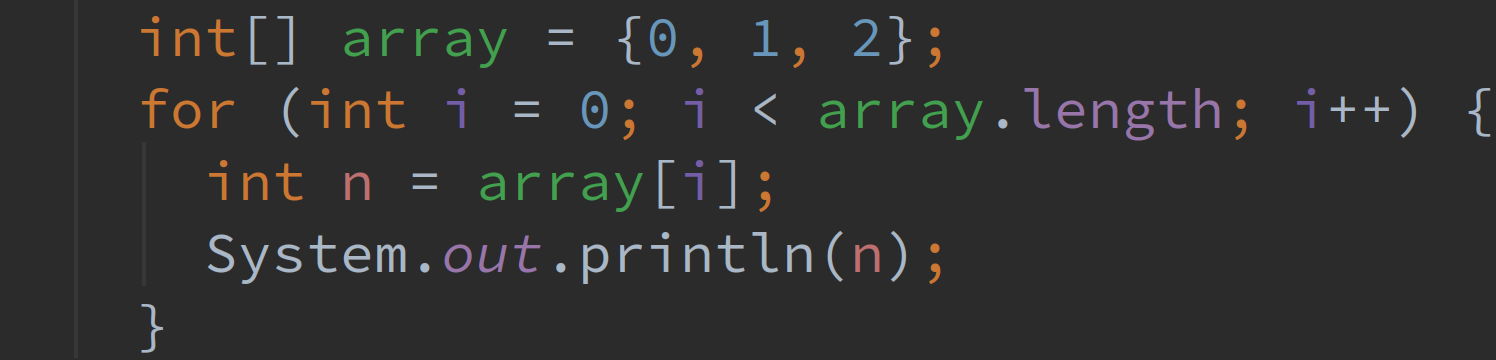
\includegraphics[height=0.625in]{src/img/foreach-to-indexed-for-after.png}
        \caption{\code{Foreach} loop to indexed \code{for} loop conversion (after) \label{img:foreach-to-indexed-for-after}}
    \end{minipage}
\end{figure}
%These two conversions are carried out using the ones that Intellij IDEA provides as intentions.